\section{Kế hoạch dự kiến cho giai đoạn 2 - Đồ Án Tốt Nghiệp}

Giai đoạn 2 (thời gian dự kiến từ tháng 1/2026 đến tháng 6/2026) nhóm sẽ tập trung hoàn thiện hệ thống, kiểm thử và triển khai. Lịch trình chi tiết được minh họa qua biểu đồ Gantt (Hình \ref{fig:gantt-chart}), với các giai đoạn chính:

\begin{itemize}
    \item \textbf{Tháng 1-2:} Refactor code theo Clean Architecture; hoàn thiện frontend cho quản lý chuyến đi, thanh toán và đánh giá (UC-02 đến UC-07, UC-13).
    \item \textbf{Tháng 2-3:} Tích hợp bản đồ Google Maps/API; xây dựng dashboard admin và hỗ trợ đa nền tảng iOS/Android (UC-10 đến UC-12).
    \item \textbf{Tháng 3-4:} Thực hiện kiểm thử đơn vị, tích hợp và end-to-end; kiểm toán bảo mật.
    \item \textbf{Tháng 4-5:} Triển khai backend/frontend; cập nhật tài liệu và báo cáo với chương triển khai, ảnh chụp màn hình.
    \item \textbf{Tháng 5-6:} Thu thập phản hồi demo, điều chỉnh; đo lường metrics và hoàn tất báo cáo cuối cùng.
\end{itemize}

Tổng thời gian: 6 tháng, với trọng tâm đảm bảo hệ thống ổn định (uptime >99.9\%) và trải nghiệm người dùng tối ưu.

\begin{figure}[H]
    \centering
    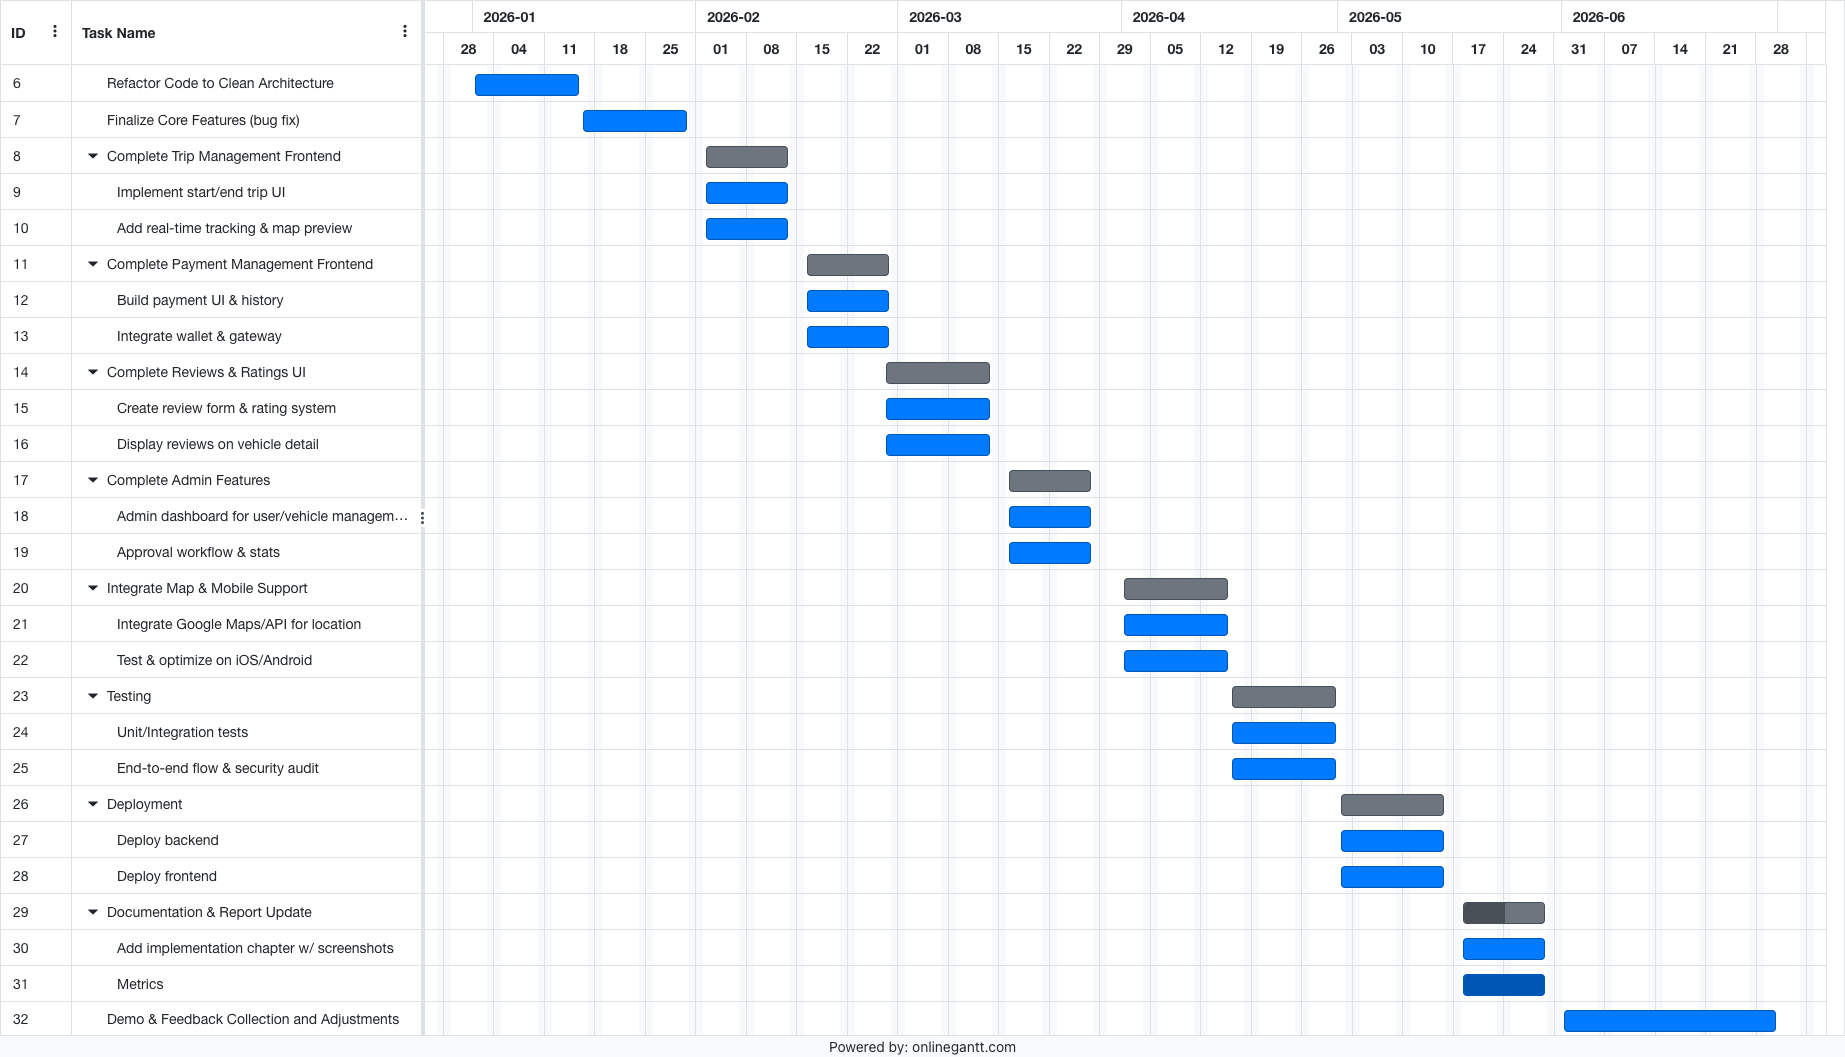
\includegraphics[width=1\textwidth]{Images/gantt-chart.png}
    \caption{Biểu đồ Gantt kế hoạch đồ án kỳ sau}
    \label{fig:gantt-chart}
\end{figure}